\documentclass[aspectratio=1610]{beamer}

\setbeamersize{text margin left=3mm,text margin right=3mm} 

\usepackage{t1enc}
\usepackage[magyar]{babel}
\usepackage{xcolor}

\definecolor{szin1}{rgb}{0.5, 0.188, 0.478}
\definecolor{szin2}{RGB}{196, 203, 133}
\definecolor{szin3}{cmyk}{0, 0.7771, 0.5437, 0.8656}
\definecolor{szin4}{gray}{0.5}

\usepackage{graphics}
\usepackage{wrapfig}

\usetheme{Malmoe}
\usecolortheme{crane}



\begin{document}

\title{Féléves beadandó}
\author{Nagy Róbert és Bartók-Balogh Gábor}
\date{\today}
\subtitle{Prezentáció  \LaTeX-kel az \textbf{xcolor} csomagról}
\institute{Miskolci Egyetem}

 % titleslide
\frame[plain]{\maketitle}

    
    % slide 1 
\begin{frame}[fragile]{Az xcolor csomag alapjai}
    \begin{minipage}{0.6\textwidth}
        \begin{itemize}
           \item \onslide<1->\verb!\usepackage[<Opciók>]{xcolor}!
           \item \onslide<2->Az xcolor lehetővé teszi, hogy kiszínezzünk 					                              szöveget,táblázatot, rajzolt ábrákat, stb... 
           \item \onslide<3->Használhatunk névvel ellátott színeket
           \item \onslide<4->Alapból 19 darab van.
           \item \onslide<5->dvipsnames opcióval 68 darab
           \item \onslide<5->svgnames opcióval 151 darab 
           \item \onslide<5->x11names opcióval pedig 317 darab
        \end{itemize}
     \end{minipage} \hfill
\begin{minipage}{0.35\textwidth}    
            \begin{figure}
                \onslide<4->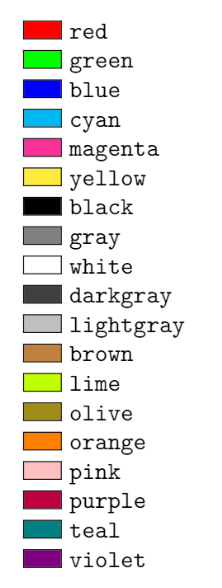
\includegraphics[scale=0.4]{img/szinek.png}
                \onslide<4->\caption{Névvel ellátott színek}
            \end{figure}
        \end{minipage}
    \end{frame}

    % slide 2
    \begin{frame}[fragile]{Az xcolor csomag alapjai}
        \begin{minipage}{0.8\textwidth}
            \begin{itemize}
                \item \onslide<1->Definiálhatunk saját színeket is.
                \item \onslide<2->\verb!\definecolor{<név>}{<Mód>}{<Értékek>}!
                \item \onslide<3->A mód lehet
                \begin{enumerate}
                    \item \onslide<4->rgb
                    \item \onslide<4->RGB
                    \item \onslide<4->cmyk
                    \item \onslide<4->gray    
                \end{enumerate}
                Például:
                \item \onslide<5->\verb!\definecolor{szin1}{rgb}{0.500, 0.188, 0.478}! \hfill \textcolor{szin1}{Szín1}
                \item \onslide<5->\verb!\definecolor{szin2}{RGB}{196, 203, 133}! \hfill \textcolor{szin2}{Szín2}
                \item \onslide<5->\verb!\definecolor{szin3}{cmyk}{0, 0.7771, 0.5437, 0.8656}! \hfill \textcolor{szin3}{Szín3}
                \item \onslide<5->\verb!\definecolor{szin4}{gray}{0.5}! \hfill \textcolor{szin4}{Szín4}
            \end{itemize}
            
        \end{minipage} 
        
    \end{frame}
\end{document}